% Record prime gaps g after p (dots; up to 10^10 computed by a segmented sieve, plus the records 1132 and 1476), against log^2 p and 2e^{-gamma} log^2 p.
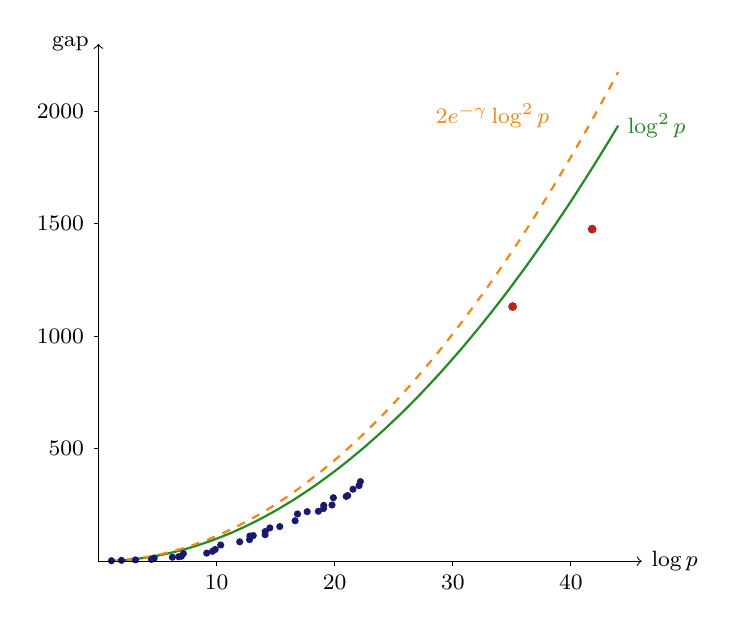
\begin{tikzpicture}[every node/.style={font=\footnotesize}]
\draw[ForestGreen,thick] (0.150,0.003)--(0.204,0.005)--(0.258,0.008)--(0.313,0.012)--(0.367,0.017)--(0.421,0.023)--(0.475,0.029)--(0.529,0.036)--(0.584,0.043)--(0.638,0.052)--(0.692,0.061)--(0.746,0.071)--(0.800,0.081)--(0.855,0.093)--(0.909,0.105)--(0.963,0.118)--(1.017,0.131)--(1.071,0.146)--(1.126,0.161)--(1.180,0.177)--(1.234,0.193)--(1.288,0.211)--(1.342,0.229)--(1.397,0.248)--(1.451,0.267)--(1.505,0.288)--(1.559,0.309)--(1.613,0.331)--(1.668,0.353)--(1.722,0.376)--(1.776,0.401)--(1.830,0.425)--(1.884,0.451)--(1.939,0.477)--(1.993,0.504)--(2.047,0.532)--(2.101,0.561)--(2.155,0.590)--(2.210,0.620)--(2.264,0.651)--(2.318,0.682)--(2.372,0.715)--(2.426,0.748)--(2.481,0.781)--(2.535,0.816)--(2.589,0.851)--(2.643,0.887)--(2.697,0.924)--(2.752,0.961)--(2.806,1.000)--(2.860,1.039)--(2.914,1.078)--(2.968,1.119)--(3.023,1.160)--(3.077,1.202)--(3.131,1.245)--(3.185,1.288)--(3.239,1.333)--(3.294,1.378)--(3.348,1.423)--(3.402,1.470)--(3.456,1.517)--(3.511,1.565)--(3.565,1.614)--(3.619,1.663)--(3.673,1.713)--(3.727,1.764)--(3.782,1.816)--(3.836,1.868)--(3.890,1.921)--(3.944,1.975)--(3.998,2.030)--(4.053,2.085)--(4.107,2.142)--(4.161,2.199)--(4.215,2.256)--(4.269,2.315)--(4.324,2.374)--(4.378,2.434)--(4.432,2.494)--(4.486,2.556)--(4.540,2.618)--(4.595,2.681)--(4.649,2.744)--(4.703,2.809)--(4.757,2.874)--(4.811,2.940)--(4.866,3.006)--(4.920,3.074)--(4.974,3.142)--(5.028,3.210)--(5.082,3.280)--(5.137,3.350)--(5.191,3.421)--(5.245,3.493)--(5.299,3.566)--(5.353,3.639)--(5.408,3.713)--(5.462,3.788)--(5.516,3.864)--(5.570,3.940)--(5.624,4.017)--(5.679,4.095)--(5.733,4.173)--(5.787,4.253)--(5.841,4.333)--(5.895,4.413)--(5.950,4.495)--(6.004,4.577)--(6.058,4.660)--(6.112,4.744)--(6.166,4.828)--(6.221,4.914)--(6.275,5.000)--(6.329,5.086)--(6.383,5.174)--(6.437,5.262)--(6.492,5.351)--(6.546,5.441)--(6.600,5.531);
\draw[BurntOrange,thick,dashed] (0.150,0.003)--(0.204,0.006)--(0.258,0.010)--(0.313,0.014)--(0.367,0.019)--(0.421,0.025)--(0.475,0.032)--(0.529,0.040)--(0.584,0.049)--(0.638,0.058)--(0.692,0.068)--(0.746,0.079)--(0.800,0.091)--(0.855,0.104)--(0.909,0.118)--(0.963,0.132)--(1.017,0.148)--(1.071,0.164)--(1.126,0.181)--(1.180,0.198)--(1.234,0.217)--(1.288,0.237)--(1.342,0.257)--(1.397,0.278)--(1.451,0.300)--(1.505,0.323)--(1.559,0.347)--(1.613,0.371)--(1.668,0.397)--(1.722,0.423)--(1.776,0.450)--(1.830,0.478)--(1.884,0.506)--(1.939,0.536)--(1.993,0.566)--(2.047,0.598)--(2.101,0.630)--(2.155,0.662)--(2.210,0.696)--(2.264,0.731)--(2.318,0.766)--(2.372,0.802)--(2.426,0.840)--(2.481,0.877)--(2.535,0.916)--(2.589,0.956)--(2.643,0.996)--(2.697,1.038)--(2.752,1.080)--(2.806,1.123)--(2.860,1.166)--(2.914,1.211)--(2.968,1.257)--(3.023,1.303)--(3.077,1.350)--(3.131,1.398)--(3.185,1.447)--(3.239,1.496)--(3.294,1.547)--(3.348,1.598)--(3.402,1.650)--(3.456,1.703)--(3.511,1.757)--(3.565,1.812)--(3.619,1.867)--(3.673,1.924)--(3.727,1.981)--(3.782,2.039)--(3.836,2.098)--(3.890,2.158)--(3.944,2.218)--(3.998,2.280)--(4.053,2.342)--(4.107,2.405)--(4.161,2.469)--(4.215,2.533)--(4.269,2.599)--(4.324,2.665)--(4.378,2.733)--(4.432,2.801)--(4.486,2.870)--(4.540,2.940)--(4.595,3.010)--(4.649,3.082)--(4.703,3.154)--(4.757,3.227)--(4.811,3.301)--(4.866,3.376)--(4.920,3.451)--(4.974,3.528)--(5.028,3.605)--(5.082,3.683)--(5.137,3.762)--(5.191,3.842)--(5.245,3.923)--(5.299,4.004)--(5.353,4.086)--(5.408,4.170)--(5.462,4.254)--(5.516,4.339)--(5.570,4.424)--(5.624,4.511)--(5.679,4.598)--(5.733,4.686)--(5.787,4.775)--(5.841,4.865)--(5.895,4.956)--(5.950,5.047)--(6.004,5.140)--(6.058,5.233)--(6.112,5.327)--(6.166,5.422)--(6.221,5.518)--(6.275,5.614)--(6.329,5.712)--(6.383,5.810)--(6.437,5.909)--(6.492,6.009)--(6.546,6.110)--(6.600,6.211);
\fill[MidnightBlue] (0.165,0.006) circle (1.3pt);
\fill[MidnightBlue] (0.292,0.011) circle (1.3pt);
\fill[MidnightBlue] (0.470,0.017) circle (1.3pt);
\fill[MidnightBlue] (0.673,0.023) circle (1.3pt);
\fill[MidnightBlue] (0.709,0.040) circle (1.3pt);
\fill[MidnightBlue] (0.939,0.051) circle (1.3pt);
\fill[MidnightBlue] (1.018,0.057) circle (1.3pt);
\fill[MidnightBlue] (1.054,0.063) circle (1.3pt);
\fill[MidnightBlue] (1.079,0.097) circle (1.3pt);
\fill[MidnightBlue] (1.375,0.103) circle (1.3pt);
\fill[MidnightBlue] (1.449,0.126) circle (1.3pt);
\fill[MidnightBlue] (1.483,0.149) circle (1.3pt);
\fill[MidnightBlue] (1.553,0.206) circle (1.3pt);
\fill[MidnightBlue] (1.794,0.246) circle (1.3pt);
\fill[MidnightBlue] (1.919,0.274) circle (1.3pt);
\fill[MidnightBlue] (1.923,0.320) circle (1.3pt);
\fill[MidnightBlue] (1.966,0.326) circle (1.3pt);
\fill[MidnightBlue] (2.117,0.337) circle (1.3pt);
\fill[MidnightBlue] (2.118,0.377) circle (1.3pt);
\fill[MidnightBlue] (2.177,0.423) circle (1.3pt);
\fill[MidnightBlue] (2.303,0.440) circle (1.3pt);
\fill[MidnightBlue] (2.498,0.514) circle (1.3pt);
\fill[MidnightBlue] (2.528,0.600) circle (1.3pt);
\fill[MidnightBlue] (2.651,0.629) circle (1.3pt);
\fill[MidnightBlue] (2.793,0.634) circle (1.3pt);
\fill[MidnightBlue] (2.859,0.669) circle (1.3pt);
\fill[MidnightBlue] (2.861,0.709) circle (1.3pt);
\fill[MidnightBlue] (2.966,0.714) circle (1.3pt);
\fill[MidnightBlue] (2.984,0.806) circle (1.3pt);
\fill[MidnightBlue] (3.147,0.823) circle (1.3pt);
\fill[MidnightBlue] (3.165,0.834) circle (1.3pt);
\fill[MidnightBlue] (3.233,0.914) circle (1.3pt);
\fill[MidnightBlue] (3.310,0.960) circle (1.3pt);
\fill[MidnightBlue] (3.327,1.011) circle (1.3pt);
\fill[BrickRed] (5.260,3.234) circle (1.6pt);
\fill[BrickRed] (6.270,4.217) circle (1.6pt);
\draw[->] (0,0)--(6.900,0) node[right] {$\log p$};
\draw[->] (0,0)--(0,6.571) node[left] {gap};
\draw (1.500,0)--(1.500,-0.06) node[below] {$10$};
\draw (3.000,0)--(3.000,-0.06) node[below] {$20$};
\draw (4.500,0)--(4.500,-0.06) node[below] {$30$};
\draw (6.000,0)--(6.000,-0.06) node[below] {$40$};
\draw (0,1.429)--(-0.06,1.429) node[left] {$500$};
\draw (0,2.857)--(-0.06,2.857) node[left] {$1000$};
\draw (0,4.286)--(-0.06,4.286) node[left] {$1500$};
\draw (0,5.714)--(-0.06,5.714) node[left] {$2000$};
\node[ForestGreen,right] at (6.600,5.531) {$\log^2p$};
\node[BurntOrange,left] at (5.850,5.660) {$2e^{-\gamma}\log^2p$};
\end{tikzpicture}
